In section \ref{subsec:general_design} we present an overview of the implementation. Afterwards, we divide the functionalities in 3 parts; in section \ref{subsec:training} we present the methods used for training (fitting) the model, in section \ref{subsec:inference} those used for performing the inference and in section \ref{subsec:evaluation} those used for evaluating the approximate posterior and the obtained samples. 

\subsubsection{General design} 
\label{subsec:general_design}
\tikzstyle{startstop} = [rectangle, rounded corners, minimum width=3cm, minimum height=1cm,text centered, draw=black, fill=red!30]
\tikzstyle{io} = [trapezium, trapezium left angle=70, trapezium right angle=110, minimum width=3cm, minimum height=1cm, text centered, draw=black, fill=blue!30]
\tikzstyle{train_process} = [rectangle, minimum width=3cm, minimum height=.7cm, text centered, draw=black, fill=green!40]
\tikzstyle{infer_process} = [rectangle, minimum width=3cm, minimum height=.7cm, text centered, draw=black, fill=blue!30]

\tikzstyle{decision} = [diamond, minimum width=.1cm, minimum height=.1cm, text centered, draw=black, fill=green!30]

\tikzstyle{public_func_rev} = [draw=black, rotate=90, anchor=north, fill=blue!20, rounded corners]
\tikzstyle{public_func} = [draw=black, fill=blue!20, rounded corners]
\tikzstyle{arrow} = [thick,->,>=stealth]


\begin{figure}[h]
  \begin{center}
  %   \resizebox{.32\textwidth}{!}{
  %     \begin{tikzpicture}[node distance=1.4cm, scale=.1]
  %     \end{tikzpicture}
  %   }
    \resizebox{.8\textwidth}{!}{    
      \begin{tikzpicture}[node distance=1.2cm, scale=.1]
        % first graph
        % private functions
        \node (n1) [train_process, xshift=-.8cm] { $\_sample\_nuisance()$  };
        \node (n2) [train_process, below of=n1] { $\_define\_objectives()$  };
        \node (n3) [decision, below of=n2, yshift=-.5cm] { $grads$  };
        \node (n4) [train_process, left of=n3, yshift=-1cm, xshift=-1.5cm] { $\_solve\_gradients()$  };
        \node (n5) [train_process, right of=n3, yshift=-1cm, xshift=1.5cm] { $\_solve\_bo()$  };
        \node (n6) [train_process, below of=n3, yshift=-1.5cm] { $\_filter\_solutions()$  };
        \node (n7) [train_process, below of=n6] { $\_build\_boxes()$  };
        \node (n8) [decision, below of=n7] { $h?$  };
        \node (n9) [train_process, right of=n8, yshift=-.5cm, xshift=1cm] { $\_fit\_models()$  };

        \node (n10) [train_process, below of=n8, yshift=-1cm] { $\_define\_posterior()$  };

        % public functions
        \node (n11) [public_func_rev, right of=n3, yshift=-5.6cm, xshift=-0.3cm, minimum width=4.7cm] {$solve\_problems()$};
        \node (n12) [public_func_rev, right of=n9, yshift=-3.4cm, xshift=-.45cm, minimum width=4.7cm] {$estimate\_regions()$};
        \node (n13) [public_func_rev, right of=n5, yshift=-4.5cm, xshift=-2.3cm, minimum width=10.5cm] {$fit\_posterior()$};
        \node (n14) [public_func, left of=n3, yshift=0.3cm, xshift=-1.5cm] {$distance\_hist()$};
        \node (n15) [public_func, left of=n6, xshift=-2.2cm, yshift=-.3cm] {$compute\_eps()$};        
        \node (n16) [public_func, left of=n7, xshift=-1.8cm, yshift=-1.5cm] {$visualize\_region()$};

        % public functions inference
        \node (n17) [public_func, below of=n10, xshift=-2cm, yshift=-.5cm] {$sample()$};
        \node (n18) [public_func, below of=n17] {$compute\_expectation()$};        
        \node (n19) [public_func, below of=n10, xshift=4cm, yshift=-.5cm] {$eval\_unnorm\_posterior()$};
        \node (n20) [public_func, below of=n19] {$eval\_posterior()$};

        % public functions evaluation
        \node (n21) [public_func, below of=n18, yshift=-.7cm] {$compute\_ess()$};
        \node (n22) [public_func, below of=n20, yshift=-.7cm] {$compute\_divergence()$};        

        % add headers
        \node (algorithm) [below of=n1, yshift=2.5cm, xshift=1cm, minimum width=4cm, minimum height=1cm] {\huge{Implementation Design} };
        
        % backgrounds
        \draw [ultra thick, draw=black, fill=yellow, opacity=0.15, rounded corners=20pt] (-115,8) rectangle (70, -108);

        \draw [ultra thick, draw=black, fill=red, opacity=0.15, rounded corners=20pt] (-115,8) rectangle (57, -48);
        \draw [ultra thick, draw=black, fill=red, opacity=0.15, rounded corners=20pt] (-115,-50) rectangle (57, -108);


        \draw [ultra thick, draw=black, fill=green, opacity=0.15, rounded corners=20pt] (-115,-110) rectangle (70, -140);

        \draw [ultra thick, draw=black, fill=cyan, opacity=0.15, rounded corners=20pt] (-115,-142) rectangle (70, -160);

        \draw [ultra thick, draw=black, fill=magenta, opacity=0.05, rounded corners=20pt] (-115,18) rectangle (-64, -160);

        \draw [ultra thick, draw=black, fill=magenta, opacity=0.05, rounded corners=20pt] (-60,18) rectangle (70, -160);
        

        % arrows
        \draw [arrow] (n1) -- (n2);
        \draw [arrow] (n2) -- (n3);
        \draw [arrow] (n3) -- (n4);
        \draw [arrow] (n3) -- (n5);
        \draw [arrow] (n4) -- (n6);
        \draw [arrow] (n5) -- (n6);
        \draw [arrow] (n6) -- (n7);
        \draw [arrow] (n7) -- (n8);
        \draw [arrow] (n8) -- (n9);
        \draw [arrow] (n9) -- (n10);
        \draw [arrow] (n8) -- (n10);


        % second graph
        \node (pro1) [train_process, left of=n1, xshift=-7cm, yshift=-1cm, minimum width=4cm, minimum height=1cm] { define $d_i(\thetab) \forall i$  };
        \node (pro2) [train_process, below of=pro1, yshift=-1cm, minimum width=4cm, minimum height=1cm] { Solve $\thetab_i^*, d_i^*, \forall i$  };
        \node (filter) [train_process, below of=pro2, yshift=-1.5cm, minimum width=4cm, minimum height=1cm] { Filter solutions  };
        \node (proposal_region) [train_process, below of=filter, yshift=-0.15cm, minimum width=4cm, minimum height=1cm] {Construct $q_i \forall i$};
        \node (surrogate) [train_process, below of=proposal_region, yshift=-0.15cm, minimum width=4cm, minimum height=1cm] {Construct $\Tilde{d}_i \forall i$};
        \node (posterior) [train_process, below of=surrogate, yshift=-0.15cm, minimum width=4cm, minimum height=1cm] {Define $p_{d,\epsilon}(\thetab)$};
        
        \node (sample) [infer_process, below of=posterior, yshift=-1.2cm, minimum width=4cm, minimum height=1cm] {Draw $\{w_{ij}, \thetab_{ij} \}$ };


        % add headers
        \node (algorithm) [below of=pro1, yshift=3.5cm, minimum width=4cm, minimum height=1cm] {\huge{Algorithm} };
        
        \draw [arrow] (pro1) -- (pro2);
        \draw [arrow] (pro2) -- (filter);
        \draw [arrow] (filter) -- (proposal_region);
        \draw [arrow] (proposal_region) -- (surrogate);
        \draw [arrow] (surrogate) -- (posterior);
        \draw [arrow] (posterior) -- (sample);

        % % backgrounds
        % \draw [ultra thick, draw=black, fill=yellow, opacity=0.15, rounded corners=5pt] (-72,8) rectangle (-62,-108);

        % % \draw [ultra thick, draw=black, fill=red, opacity=0.15, rounded corners=20pt] (-60,8) rectangle (57, -48);
        % % \draw [ultra thick, draw=black, fill=red, opacity=0.15, rounded corners=20pt] (-60,-50) rectangle (57, -108);


        % % \draw [ultra thick, draw=black, fill=green, opacity=0.15, rounded corners=20pt] (-60,-110) rectangle (70, -140);

        % % \draw [ultra thick, draw=black, fill=cyan, opacity=0.15, rounded corners=20pt] (-60,-142) rectangle (70, -160);

        
        % \draw [arrow] (pro1) -- (pro2);
        % \draw [arrow] (pro2) -- (filter);
        % \draw [arrow] (filter) -- (proposal_region);
        % \draw [arrow] (proposal_region) -- (surrogate);

        
      \end{tikzpicture}
    }
  \end{center}
  \caption{Overview of the
ROMC implementation. The training part follows a sequential pattern;
the functions in the green ellipses must be called in a sequential
fashion for completing the training part and define the posterior
distribution. The functions in blue ellipses are the functionalities
provided to the user.}
\end{figure}


The overview of our implementation is illustrated in
figure~\ref{fig:romc_overview}; one may interpret
figure~\ref{fig:romc_overview} as a depiction of the main class and
the ellipses are the main routines of the class. Following
\proglang{Python}'s naming principles, the methods starting with an
underscore (green ellipses) represent internal (private) functions,
whereas the rest (blue ellipses) are the public methods that the user
interacts with. In figure~\ref{fig:romc_overview}, it can be easily
observed that the implementation follows consistently the algorithmic
view presented in~\ref{alg:romc_algorithm}. The training part includes
all the steps until the computation of the proposal regions
i.e. sampling the nuisance variables, defining the optimization
problems, solving them, constructing the regions and fitting local
surrogate models. The inference part comprises of evaluating the
unnormalized posterior (and the normalized when is possible), sampling
and computing an expectation. We also provide some utilities for
inspecting the training process, such as plotting the histogram of the
final distances or visualizing the constructed bounding
boxes. Finally, in the evaluation part, we provide two methods for
evaluating the inference; (a) computing the Effective Sample Size
(ESS) of the samples and (b) measuring the divergence between the
approximate posterior the ground-truth, if the latter is
available.\footnote{Normally, the ground-truth posterior is not
  available; However, this functionality is useful in cases where the
  posterior can be computed numerically or with an alternative method
  (i.e.\ ABC Rejection Sampling), and we would like to measure the
  discrepancy between the two approximations.}

\subsubsection*{Parallelizing ROMC method}

ROMC has the significant advantage of being fully parallelizable. We
exploit this fact by implementing a parallel version of all the major
components of the method; (a) solving the optimization problems, (b)
constructing bounding box regions, (c) sampling and (d) evaluating the
posterior. We parallelize these processes using the built-in
\proglang{Python} package \pkg{multiprocessing}. The specific package
enables concurrency, using subprocesses instead of threads, for
side-stepping the Global Interpreter (GIL). For activating the
parallel version of the algorithm, the user simpy has to pass the
argument \code{parallelize=True} when instantiating \code{ROMC}.

\begin{Code}
---------------------------------- python ----------------------------------
>>> elfi.ROMC(<output_node>, parallelize=True)
----------------------------------------------------------------------------
\end{Code}
  
\subsubsection*{Simple one-dimensional example}

For illustrating the functionalities we will use the following running
example introduced by~\cite{Ikonomov2019},

\begin{gather} \label{eq:1D_example}
  p(\theta) = \mathcal{U}(\theta;-2.5,2.5)\\ \label{eq:1D_example_eq_2}
  p(y|\theta) = \left\{
    \begin{array}{ll} \theta^4 + u & \mbox{if } \theta \in [-0.5, 0.5]
\\ |\theta| - c + u & \mbox{otherwise}
    \end{array} \right.\\ 
  u \sim \mathcal{N}(0,1)
\end{gather}

\noindent

The prior is a uniform distribution in the range $[-2.5, 2.5]$ and the
likelihood is defined at~\ref{eq:1D_example_eq_2}. There is only one
observation $y_0 = 0$. The inference in this particular example can be
performed quite easily without using a likelihood-free inference
approach. We can exploit this fact for validating the accuracy of our
implementation.

In the following code snippet, we code the model at \pkg{ELFI}.

\begin{Code}
------------------------------ python snippet ------------------------------
  import elfi import scipy.stats as ss
  import numpy as np

  def simulator(t1, batch_size=1,random_state=None):
    if t1 < -0.5:
        y = ss.norm(loc=-t1-c, scale=1).rvs(random_state=random_state)
    elif t1 <= 0.5:
        y = ss.norm(loc=t1**4, scale=1).rvs(random_state=random_state)
    else:
        y = ss.norm(loc=t1-c, scale=1).rvs(random_state=random_state)
    return y

  # observation
  y = 0
      
  # Elfi graph
  t1 = elfi.Prior('uniform', -2.5, 5)
  sim = elfi.Simulator(simulator, t1, observed=y)
  d = elfi.Distance('euclidean', sim)

  # Initialise the ROMC inference method
  bounds = [(-2.5, 2.5)] # limits of the prior
  parallelize = True # activate parallel execution
  romc = elfi.ROMC(d, bounds=bounds, parallelize=parallelize)
----------------------------------------------------------------------------
\end{Code}


\subsubsection{Training part} 
\label{subsec:training}
The training part contains six methods.

\begin{Code}
---------------------------------- python ----------------------------------
>>> romc.solve_problems(n1,
                        use_bo=False,
                        optimizer_args=None,
                        seed=None)
----------------------------------------------------------------------------                    
\end{Code}


\noindent
This method (a) draws the nuisance variables, (b) defines the
optimisation problems and (c) solves them using either a
gradient-based optimizer or Bayesian optimization. These tasks are
compleed sequentially, as shown in figure~\ref{fig:romc_overview}. The
definition of the optimisation problems is performed by drawing
\code{n_1} integer numbers from a discrete uniform distribution
$u_i \sim \mathcal{U}\{1, 2^{32}-1\}$. Each integer $u_i$ is the seed
used in \pkg{ELFI}'s random simulator. The seed $u_i$ is the
computational analogous of the random variables $\vb_i$, that were
defined in the previous chapter; freezing the \code{seed} absorbs all
the randomness of the simulator transforming it to a deterministic
function. Setting the argument \code{use_bo=True}, chooses the
Bayesian Optimisation scheme for obtaining $\thetab_i^*$. In this
case, apart from obtaining the optimal points $\thetab_i^*$, we also
fit a Gaussian Process (GP) as surrogate model $\hat{d}_i$. In this
scenario, in the following steps, $\hat{d}_i(\thetab)$ will replace
$g_i(\thetab)$ as the distance function.

\begin{Code}
---------------------------------- python ----------------------------------
>>> romc.distance_hist(**kwargs)
----------------------------------------------------------------------------  
\end{Code}

\noindent
This function helps the user decide which threshold $\epsilon$ to
use. It plots a histogram of the distances at the optimal point
$g_i(\thetab_i^*) : \{i = 1, 2, \ldots, n_1\}$ or $d_i^*$ in case
\code{use_bo=True}. The function accepts all keyword arguments and
forwards them to the underlying \code{matplotlib.hist()} function; in
this way the user may customise some properties of the histogram, such
as the number of bins or the range of values.

\begin{Code}
---------------------------------- python ----------------------------------  
>>> romc.estimate_regions(eps_filter,
                          use_surrogate=None,
                          region_args=None,
                          fit_models=False,
                          fit_models_args=None,
                          eps_region=None,
                          eps_cutoff=None)
----------------------------------------------------------------------------
\end{Code}

\noindent
This method constructs a bounding box around the optimal point
$\thetab_i^* : i = 1, 2, \ldots, n_1$ following
Algorithm~\ref{alg:region_construction}. The Hessian matrix is
approximated based on the Jacobian $\hess_i = \jac_i^T \jac_i$. The
eigenvectores are computed using the function
\code{numpy.linalg.eig()}. A check is performed so that the matrix
$\hess_i$ is not singular; if this is the case, the eigenvectors are
set to be the vectors of the standard Euclidean basis i.e.\
$\{ \mathbf{e_1} = (1, 0, \ldots), \mathbf{e_2} = (0,1,0,\ldots),
\text{etc} \}$. The limits of the bounding box are obtained by
repeteadly querying the distance function ($g_i(\thetab)$ or
$\hat{d}(\thetab)$) along the search directions given by $\hess_i$.

\begin{Code}
---------------------------------- python ----------------------------------
>>> romc.fit_posterior(n1,
                       eps_filter,
                       use_bo=False,
                       optimizer_args=None,
                       seed=None,
                       use_surrogate=None,
                       region_args=None,
                       fit_models=False,
                       fit_models_args=None,
                       eps_region=None,
                       eps_cutoff=None)
----------------------------------------------------------------------------
\end{Code}

\noindent
The function \code{fit_posterior} is a syntactic sugar for applying
\code{solve_problems} and \code{estimate_regions} into a single
step. 

% merges all steps for constructing the bounding box into
% a single command. If the user doesn't want to manually inspect the
% histogram of the distances before deciding where to set the threshold
% $\epsilon$, he may call \code{romc.fit_posterior()} and the whole
% training part will be done end-to-end. There are two alternatives for
% setting the threshold $\epsilon$; the first is to set to a specific
% value blindly, and the second is to set at as a specific quantile of
% the histogram of distances. In the second scenario the
% \code{quantile} argument must be set to a floating number in the
% range $[0,1]$ and \code{eps='auto'}.


\begin{Code}
---------------------------------- python ----------------------------------
>>> romc.visualize_region(i)
----------------------------------------------------------------------------
\end{Code}

\noindent

It can be used for plotting the bounding box around the optimal point,
when the parameter space is $1D$ or $2D$. The argument \code{i} is the
index of the corresponding optimization problem i.e.\ $i<n_1$.

\begin{Code}
---------------------------------- python ----------------------------------  
>>> romc.compute_eps(quantile)
----------------------------------------------------------------------------
\end{Code}

\noindent
This function return the appropriate distance value $d_{i=\kappa}^*$
where $\kappa = \lfloor \frac{quantile}{n} \rfloor$ from the
collection $\{ d_i^* \} \forall i = \{1, \ldots, n\}$ where $n$ is the
number of accepted solutions. It can be used to automate the selection
of the threshold $\epsilon$, e.g.\
\code{eps=romc.compute_eps(quantile=0.9)}.


\subsubsection*{Example}


In the following snippet, we put together the routines described above
to perform the training part at our running example.

\begin{Code}
------------------------------ python snippet ------------------------------  
  n1 = 500 # number of optimisation problems
  seed = 21 # seed for solving the optimisation problems
  eps = .75 
  use_bo = False # set to True for switching to Bayesian optimisation

  # Training step-by-step
  romc.solve_problems(n1=n1, seed=seed, use_bo=use_bo)
  romc.theta_hist(bins=100) # plot hist to decide which eps to use

  eps = .75 # threshold for the bounding box based on histogram inspection
  romc.estimate_regions(eps=eps) # build the bounding boxes

  romc.visualize_region(i=1) # for inspecting visually the bounding box

  # Equivalent one-line command
  # romc.fit_posterior(n1=n1, eps=eps, use_bo=use_bo, seed=seed)
----------------------------------------------------------------------------  
\end{Code}

In figure \ref{fig:example_training_hist} we illustrate the
distribution of the distances obtained and the acceptance area of the
first optimisation problem. We observe that most optimal points
produce almost zero distance.

\begin{figure}[h]
  \begin{center}
    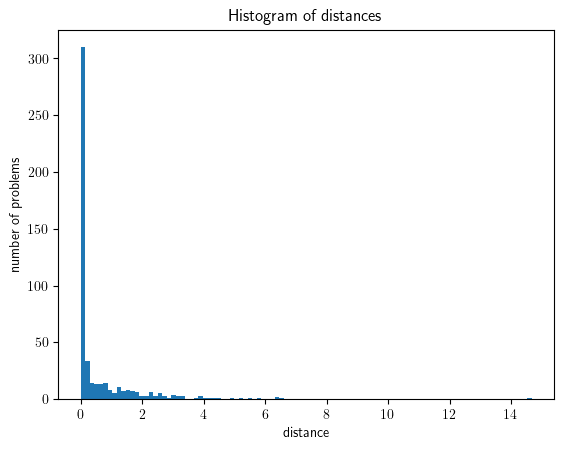
\includegraphics[width=0.48\textwidth]{./latex_files/images/chapter3/example_theta_dist.png}
    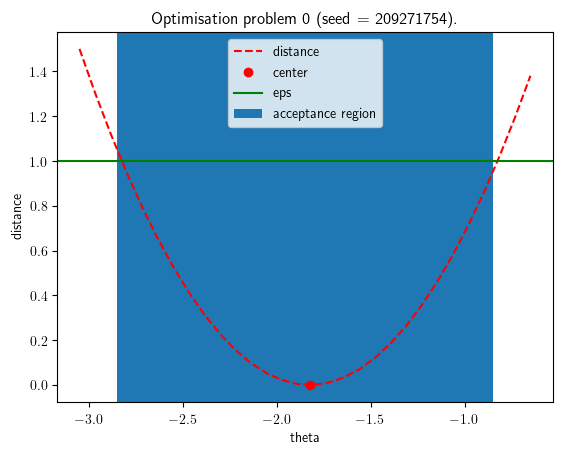
\includegraphics[width=0.48\textwidth]{./latex_files/images/chapter3/example_region.png}
    \end{center}
    \caption[Histogram of distances at the 1D example.]{Histogram of
      distances and visualisation of a specific region.}
    \label{fig:example_training_hist}
\end{figure}


\subsubsection{Inference part} 
\label{subsec:inference}
The inference part contains the 4 following functionalities:

\begin{enumerate}
\item \mintinline{python}{romc.sample(n2, seed=None)}
\item \mintinline{python}{romc.compute_expectation(h)}  
\item \mintinline{python}{romc.eval_unnorm_posterior(theta)}
\item \mintinline{python}{romc.eval_posterior(theta)}
\end{enumerate}

\subsubsection*{Function (i): Perform weighted sampling}

\mintinline{python}{romc.sample(n2)}
\vspace{5mm}

\noindent
This is the basic inference utility of the ROMC implementation; we
draw $n_2$ samples for each bounding box region. This gives a total of
$k \times n_2$, where $k < n_1$ is the number of the optimal points
remained after filtering\footnote{From the $n_1$ optimisation
  problems, only the ones with $g_i(\thetab_*) < \epsilon$ are kept
  for building a bounding box}. The samples are drawn from a uniform
distribution $q_i$ defined over the corresponding bounding box and the
weight $w_i$ is computed as in equation~\eqref{eq:sampling}. The
function stores an \pinline{elfi.Result} object as
\pinline{romc.result} attribute. The \pinline{elfi.Result} provides
some usefull functionalities for inspecting the obtained samples e.g.\
\pinline{romc.result.summary()} prints the number of the obtained
samples and their mean. A complete overview of these functionalities is
provided in ELFI's
\href{https://elfi.readthedocs.io/en/latest/api.html#elfi.methods.results.Sample}{official
  documentation}.

\subsubsection*{Function (ii): Compute an expectation}

\mintinline{python}{romc.compute_expectation(h)}
\vspace{5mm}

\noindent
This function computes the expectation
$E_{p(\thetab|\data)}[h(\thetab)]$ using
expression~\eqref{eq:expectation}. The argument \pinline{h} can be
any python \pinline{Callable}.

\subsubsection*{Function (iii): Evaluate the unnormalised posterior}
\mintinline{python}{romc.eval_unorm_posterior(theta, eps_cutoff=False)}
\vspace{5mm}

\noindent
This function computes the unnormalised posterior approximation using
expression~\eqref{eq:approx_posterior}.

\subsubsection*{Function (iv): Evaluate the normalised posterior}
\mintinline{python}{romc.eval_posterior(theta, eps_cutoff=False)}
\vspace{5mm}

\noindent
This function evaluates the normalised posterior. For doing so it
needs to approximate the partition function
$Z = \int p_{d,\epsilon}(\thetab|\data)d\thetab$; this is done using
the Riemann integral approximation. Unfortunately, the Riemann
approximation does not scale well in high-dimensional spaces, hence
the approximation is tractable only at low-dimensional parametric
spaces. Given that this functionality is particularly useful for
plotting the posterior, we could say that it is meaningful to be used
for up to $3D$ parametric spaces, even though it is not restricted to
that. Finally, for this functionality to work, the \pinline{bounds}
arguments must have been set at the initialisation of the
\pinline{elfi.ROMC} object.\footnote{The argument \pinline{bounds}
  should define a bounding box \emph{containing} all the mass of the
  prior; it may also contain redundant areas. For example, if the
  prior is the uniform defined over a unit circle i.e.\
  $c=(0,0), r=1$, the best bounds arguments is
  \pinline{bounds=[(-1,1),(-1,1)]}. However, any argument
  \pinline{bounds=[(-t,t),(-t,t)]} where $t\geq1$ is technically
  correct.}

\subsubsection*{Example - Sampling and compute expectation}

With the following code snippet, we perform weighted sampling from the
ROMC approximate posterior. Afterwards, we used some ELFI's built-in
tools to get a summary of the obtained samples. In figure
\ref{fig:example_sampling}, we observe the histogram of the weighted
samples and the acceptance region of the first deterministic function
(as before) alongside with the obtained samples obtained from
it. Finally, in the code snippet we demonstrate how to use the
\pinline{compute_expectation} function; in the current example we
define \pinline{h} in order to compute firstly the empirical mean and
afterwards the empirical variance. In both cases, the empirical result
is close to the ground truth $\mu = 0$ and $\sigma^2 = 1$.

\begin{pythoncode}
  seed = 21
  n2 = 50
  romc.sample(n2=n2, seed=seed)

  # visualize region, adding the samples now
  romc.visualize_region(i=1)

  # Visualise marginal (built-in ELFI tool)
  romc.result.plot_marginals(weights=romc.result.weights, bins=100, range=(-3,3))

  # Summarize the samples (built-in ELFI tool)
  romc.result.summary()
  # Number of samples: 1720
  # Sample means: theta: -0.0792

  # compute expectation
  print("Expected value   : %.3f" % romc.compute_expectation(h=lambda x: np.squeeze(x)))
  # Expected value   : -0.079

  print("Expected variance: %.3f" % romc.compute_expectation(h=lambda x: np.squeeze(x)**2))
  # Expected variance: 1.061
\end{pythoncode}

\begin{figure}[h]
    \begin{center}
      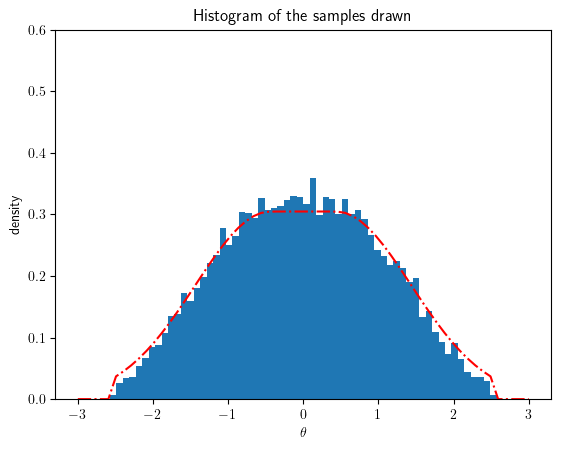
\includegraphics[width=0.48\textwidth]{./latex_files/images/chapter3/example_marginal.png}
      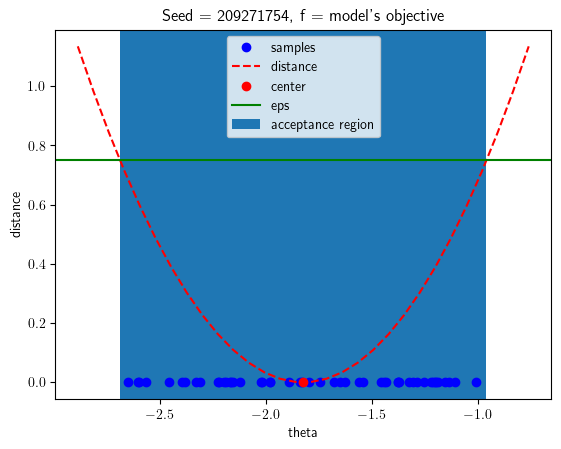
\includegraphics[width=0.48\textwidth]{./latex_files/images/chapter3/example_region_samples.png}
    \end{center}
  \caption[Histogram of the obtained samples at the 1D example.]{(a) Left: Histogram of the obtained samples. (b) Right: Acceptance region around $\theta_1^*$ with the obtained samples plotted inside.}
  \label{fig:example_sampling}
\end{figure}

\subsubsection*{Example - Evaluate Posterior}

The \pinline{romc.eval_unnorm_posterior(theta)} evaluates the
posterior at point $\theta$ using expression
\eqref{eq:aprox_posterior}. The \pinline{romc.eval_posterior(theta)}
approximates the partition function
$Z = \int_{\thetab} p_{d,\epsilon}(\thetab|\data) d\thetab$ using the
Riemann approximation as explained above. In our simple example, this
utility can provide a nice plot of the approximate posterior as
illustrated in figure~\ref{fig:approx_posterior}. We observe that the
approximation is quite close to the ground-truth posterior.

\begin{figure}[ht]
    \begin{center}
      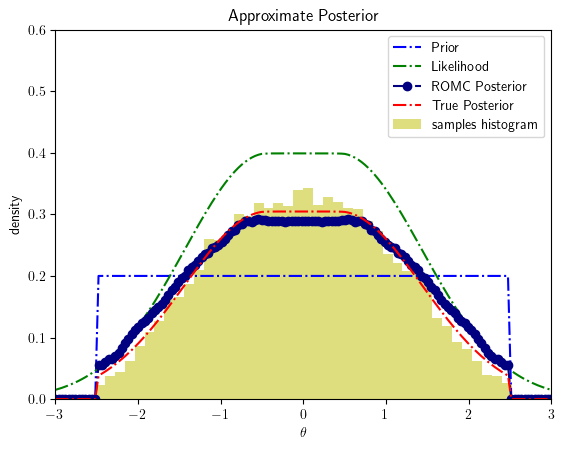
\includegraphics[width=0.75\textwidth]{./latex_files/images/chapter3/example_posterior.png}
    \end{center}
  \caption[Approximate posterior evaluation, at the 1D example.]{Approximate posterior evaluation.}
  \label{fig:approx_posterior}
\end{figure}


\subsubsection{Evaluation part} 
\label{subsec:evaluation}
The ROMC implementation provides two functions for evaluating the inference results.

\begin{Code}
---------------------------------- python ----------------------------------  
>>> romc.compute_divergence(gt_posterior,
                            bounds=None,
                            step=0.1,
                            distance="Jensen-Shannon")
----------------------------------------------------------------------------
\end{Code}

\noindent
This function computes the divergence between the ROMC approximation
and the ground truth posterior. Since the computation is performed
using the Riemann's approximation, this method can only work in low
dimensional parameter spaces; it is suggested to be used for up to the
three-dimensional parameter space. As mentioned at the beginning of
this chapter, in a real-case scenario it is not expected the
ground-truth posterior to be available. However, in cases where the
posterior can be approximated decently well with a numerical approach
(as in the current example) or with some other inference approach,
this function can provide a numerical measure of the agreement between
the two approximations. The argument \code{step} defines the step used
in the Riemann's approximation and the argument \code{distance} can
take either the \code{Jensen-Shannon} or the \code{KL-divergence}
value, for computing the appropriate distance.

\begin{Code}
---------------------------------- python ----------------------------------  
>>> romc.compute_ess()
----------------------------------------------------------------------------
\end{Code}

\noindent
This function computes the Effective Sample Size (ESS) using the
following expression~\cite{Sudman1967},

\begin{equation} \label{eq:ESS}
  ESS = \frac{(\sum_i w_i)^2}{\sum_i w_i^2}
\end{equation}

The ESS is a valuable measure of the \textbf{actual} sample size when
the samples are weighted. For example, if in a population of $100$
samples one has an enormous weight (e.g.\ $\approx 100$) whereas the
rest have small (i.e.\ $\approx 1$), the actual sample size is close
to 1; one sample dominates over the rest. Hence, the ESS provides a
measure of the equivalent uniformly weighted sample population.



\begin{Code}
------------------------------ python snippet ------------------------------  
  res = romc.compute_divergence(wrapper, distance="Jensen-Shannon")                                 
  print("Jensen-Shannon divergence: %.3f" % res)
  # Jensen-Shannon divergence: 0.025

  nof_samples = len(romc.result.weights)
  ess = romc.compute_ess()
  print("Nof Samples: %d, ESS: %.3f" % (nof_samples, ess))
  # Nof Samples: 19950, ESS: 16694.816
----------------------------------------------------------------------------  
\end{Code}

